\documentclass[a4paper,12pt,titlepage]{article}

%% On charge quelques paquets
\usepackage[utf8]{inputenc}
\usepackage[T1]{fontenc}
\usepackage[french]{babel}
\usepackage{amsfonts}
\usepackage{amsmath}
\usepackage{amsthm}
\usepackage{amssymb}
\usepackage{graphicx}
\usepackage{hyperref}
\usepackage{wrapfig}
%% quelques définitions
\theoremstyle{plain}
\newtheorem{thm}{Théorème}
\newtheorem{cor}[thm]{Corollaire}
\newtheorem{lem}[thm]{Lemma}
\newtheorem{prop}{Proposition}
\newtheorem{dem}{Démonstration}

%raccourci
\newcommand{\Ftrois}[1]{\mathbb{F}^#1_3}
%\newcommand{\F}[1]{\mathbb{F}^#1_3}

\theoremstyle{definition}
\newtheorem{defi}{Définition}
\newtheorem{rmq}{Remarque}
\newtheorem{ex}{Exemple}
\newtheorem{exo}{exercice}

\title{Projet de mathématiques \\
		\large Interprétation géométrique des règles du jeu de SET}
\author{Nathan C. \and Romain B.}
%\date{}

%% on commence
\begin{document}

\maketitle
\tableofcontents
\newpage

\begin{abstract}
Dans ce sujet, on verra comment interpréter les règles du jeu de SET de manière géométrique, 
puis grâce à cette interprétation comment déterminer le nombre de cartes minimal à disposer devant soi pour pouvoir toujours trouver un triplet de cartes.
\end{abstract}




\section{Présentation du jeu de SET}
\subsection{Origine}
Le Jeu de SET a été inventé par Marsha Falco en 1974. L'idée du jeu est venue lorsque Marsha essayait de comprendre si l'épilepsie chez les bergers allemands était héritée. 
Elle représentait les données génétiques des chiens sous la forme de symboles en dessinant sur des fiches. 
Marsha a constaté qu'il était amusant de trouver les différentes combinaisons et SET est né. Au fil des années, Marsha a perfectionné le jeu en jouant avec sa famille et ses amis. 
Il a finalement été lancé en 1990.

\subsection{But}
Chaque joueur doit trouver le maximum de sets. Un set est composé de trois cartes dont les quatre caractéristiques (prises séparément) sont : 
\begin{itemize}
\item soit totalement identiques (par exemple les trois cartes ont la même forme),
\item soit totalement différentes (par exemple chacune des trois cartes est d'une couleur différente).
\end{itemize}

\subsection{Règles}
Le jeu commence en disposant douze cartes devant les joueurs.
Le premier joueur qui voit un set prend les trois cartes et les garde dans sa pile de gain. 
On complète avec trois cartes de la pioche. Si aucun set ne figure parmi les 12 cartes, on ajoute 3 cartes, mais on ne complètera pas après qu'un joueur a trouvé une solution.
Le jeu est fini quand toutes les cartes ont été tirées et qu'il n'y a plus de set dans celles qui restent.
Le gagnant est celui qui a le plus grand nombre de sets. 

\section{Notions mathématique utilisées}
Avant d'aborder l'aspect mathématique du jeu de set, en particulier l'interprétation géométrique des règles; nous allons expliquer et illustrer les notions de mathématique indispensables à la compréhension de la section suivante. 

\subsection{Le corps fini $\mathbb{F}_3$}
Le corps commutatif fini $\mathbb{F}_3$ est composé de trois éléments distincts qui sont 0,1 et 2. Il peut s'interpréter comme l'anneau $\mathbb{Z}/3\mathbb{Z}$ correspondant au calcul modulaire sur les restes des entiers dans la division par 3. Un élément de $\mathbb{Z}/3\mathbb{Z}$ est la classe des éléments ayant tous le même reste par la division euclidienne par 3, cet élément est identifié par un membre de sa classe.
\begin{ex}
$\bar{2}$ représente la classe contenant les éléments $5,8,11$ etc. Comme il n'y a pas d'ambigüité, 2 désignera aussi cette classe.
\end{ex}

\begin{rmq}
Notons que comme 3 est un nombre premier chaque élément non nul de $\mathbb{F}_3$ est inversible, c'est l'inverse modulaire. L'inverse modulaire d'un entier relatif $a$ pour la multiplication modulo $n$ est un entier $u$ satisfaisant l'équation $au \equiv 1 \pmod{n}$.
\end{rmq}

Les lois $(+,\times)$ sont les mêmes que sur $\mathbb{Z}$ mais modulo 3.
\begin{center}
\begin{tabular}{ l | c c c }
+ & 0 & 1 & 2 \\
\hline
0 & 0 & 1 & 2\\
1 & 1 & 2 & 0\\
2 & 2 & 0 & 1\\
\end{tabular}
\qquad
\begin{tabular}{ l | c c c }
$\times$ & 0 & 1 & 2 \\
\hline
0 & 0 & 0 & 0\\
1 & 0 & 1 & 2\\
2 & 0 & 2 & 1\\
\end{tabular}
\end{center}
\subsubsection{Considérations graphiques}
\'{E}tant donné que nous sommes modulo 3, le plan $\Ftrois{2}$ se comporte comme un tore.

GRAPHIQUE

\subsection{Relation d'équivalence et classe d'équivalence}
\subsubsection{Relation d'équivalence}
La relation d'équivalence permet, dans un ensemble, de mettre en relation des éléments qui sont similaires par une certaine propriété.
\begin{defi}
Une relation d'équivalence sur un ensemble E est une relation binaire $\sim$ sur E qui est à la fois réflexive, symétrique et transitive.
\end{defi}
\begin{ex}
Dans $\mathbb{Z}/3\mathbb{Z}$ la relation d'équivalence correspond à la congruence sur les entiers. On vérifie aisément que la congruence est réflexive, symétrique et transitive.
\end{ex}
\subsubsection{Classe d'équivalence}
Grâce à la relation d'équivalence, on peut regrouper des éléments équivalents, similaires ensembles, on définit ainsi la notion de classe d'équivalence.
\begin{defi}
On définit la classe d'équivalence [x] d'un élément $x$ de $E$ comme l'ensemble des $y$ de $E$ tels que $x \sim  y$, autrement dit, on a $y \in [x] \Leftrightarrow x \sim  y$.
\end{defi}
On appelle représentant de [x] n'importe quel élément de [x]. On a par ailleurs $x \sim  y \Leftrightarrow  [y] = [x]$.
\begin{ex}
-1, 2, 5, etc sont des représentants de $[2]=\{x \equiv 2 \pmod{3}~|~x \in \mathbb{Z}\}$.
\end{ex}

\subsection{Espace vectoriel quotient}
\subsection{Espace affine}
\section{Aspect Mathématique}
\subsection{Combinatoire}

\paragraph{Nombre de cartes} Chaque carte du jeu de SET est unique, en effet une carte représente une combinaison de quatre attributs, chacun des attributs pouvant prendre trois valeurs. 
Il y a donc $3^4=81$ cartes dans le jeu de SET.

\paragraph{Probabilité d'obtenir un set en tirant 3 cartes au hasard} Avant de calculer la probabilité, il est important d'énoncer le théorème suivant :

\begin{thm}[Théorème de construction d'un Set]\label{thm:Construction}
Pour deux cartes, il y a exactement une carte qui complète ces deux cartes en un set.
\end{thm}
\begin{proof}
Par définition, si les deux cartes ont la même forme alors la troisième carte a cette forme sinon les deux cartes n'ont pas la même forme alors la troisième carte a une forme différentes des deux autres. On cherche ainsi une carte vérifiant cette condition pour la forme et pour les autres attributs.
\end{proof}
D'après le théorème précédent, après avoir tiré deux cartes la troisième existe parmi les 79 cartes restantes. On en déduit qu'on a une probabilité de 1/79 d'obtenir un set en tirant 3 cartes aléatoirement.

\paragraph{Nombre de sets dans le jeu} On tire une première carte parmi les 81 cartes, puis une deuxième parmi les 80 cartes restantes, d'après le théorème \ref{thm:Construction} la troisième carte complétant le set est unique. 
De plus, on ne compte pas les permutations possibles des cartes tirées, on a alors $\frac{81 \times 80 \times 1}{3!} = 1080$ sets possibles dans le jeu.

\subsection{Interprétation géométrique des règles}
Chaque carte possède quatre attributs pouvant prendre trois valeurs différentes. On peut alors dire qu'un attribut est représenté par un élément appartenant  à $\mathbb{F}_3$, un corps commutatif fini composé de trois éléments : 0,1,2.
De plus, une carte possède quatre attributs, il y aura donc quatre dimensions (une pour chaque attribut). Une carte est alors représentée par un unique point $(x_1,x_2,x_3,x_4) \in \Ftrois{4}$.
On peut ainsi poser le tableau suivant :

\begin{center}
\begin{tabular}{r l | c c c }
 & & 0 & 1 & 2 \\
\hline
$x_1$: & Nombres     & un		& deux	  & trois 	\\
$x_2$: & Remplissage & plein 	& hachuré & vide 	\\
$x_3$: & Couleur     & rouge	& vert	  & violet 	\\
$x_4$: & Forme       & ovale	& vague	  & losange \\
\end{tabular}
\end{center}

\begin{ex}
Le point de coordonnées $(1,0,1,2)$ représente la carte : 
\includegraphics[width=0.1\textwidth]{Img/1012.png}.
\end{ex}

Sous cette formulation, on obtient la proposition suivante :
\begin{prop}
Trois cartes forment un set si et seulement si leur point représentatif dans  $\Ftrois{4}$ sont alignés.
\end{prop}
\begin{proof}
Soit $\lambda_1,\lambda_2,\lambda_3 \in \mathbb{F}_3$. On a $\lambda_1 + \lambda_2 + \lambda_3 = 0$ si et seulement si $\lambda_1=\lambda_2=\lambda_3$ ou $\lambda_1,\lambda_2$ et $\lambda_3$ sont tous différents. Pour des points $a,b,c$ appartenant à  $\Ftrois{4}$, avoir $a+b+c=0$ signifie que toutes les coordonnées sont soit identiques ou soit différentes.
Pour $a,b,c$ des points de  $\Ftrois{4}$, on a $a+b+c=0 \iff a-2b+c=0 \iff a-b=b-c$ donc les trois points sont alignés.
\end{proof}


\subsection{Taille maximale d'un \emph{cap}}
\begin{defi}[d-cap]
On appelle \emph{d-cap} un sous-espace de  $\Ftrois{d}$ ne contenant pas trois points alignés. \\
\end{defi}
Nous nous posons la question : Combien de cartes au minimum doit-on disposer devant soi pour être certain d'avoir un set ?
Cela revient, entre autre, à chercher la taille maximale d'un 4-cap. D'après la séquence A090245 de l'\emph{OEIS}\footnote{L'Encyclopédie en ligne des suites de nombres entiers} la taille maximale d'un 4-cap est 20, il faudra alors disposer au minimum 21 cartes devant soi pour avoir un set.
Avant de démontrer ce résultat, nous étudierons des variantes du jeu de SET en considérant, par exemple, une couleur fixée pour toutes les cartes. Autrement dit, nous travaillerons d'abord dans des sous-espaces de  $\Ftrois{4}$.

\subsubsection{Taille maximale d'un \emph{2-cap}}
\begin{prop} \label{prop:2cap}
La taille maximale d'un \emph{2-cap} est 4.
\end{prop}
\begin{proof}  
Par l'absurde, supposons qu'il existe un 2-cap représenté avec 5 points que l'on note $x_1,x_2,x_3,x_4,x_5$. Le plan $\mathbb{F}_3^d$ peut être décomposé en unissant trois lignes parallèles horizontales. La figure \ref{fig:F32decomp} représente cette décomposition.

\begin{figure}[h!] \label{fig:F32decomp}
\centering
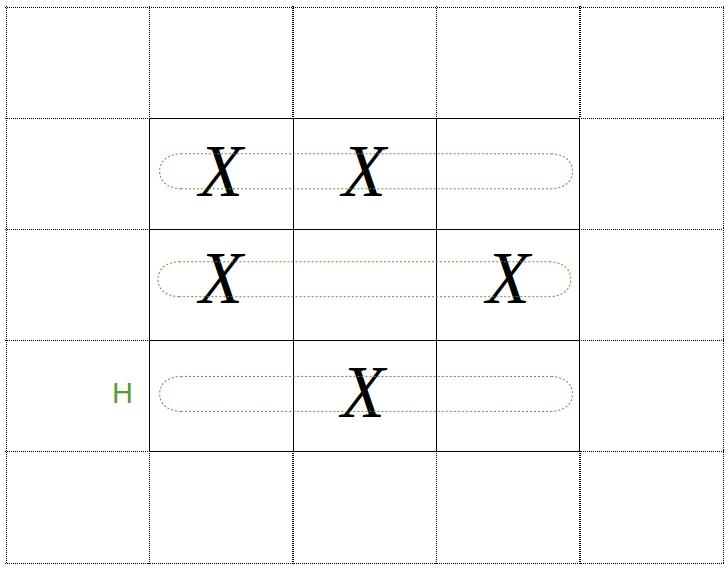
\includegraphics[width=0.5\textwidth]{Img/FigProp1v2.jpg}
\caption{Décomposition de $\Ftrois{2}$ comme l'union de trois droites horizontales parallèles}
\end{figure}

Chaque ligne contient au plus 2 points, par conséquent il existe deux lignes horizontales contenant chacune deux points du cap et une autre ligne, notée $H$, qui contient exactement un point qui sera le point $x_5$. Finalement, il y a exactement 4 lignes contenant le point $x_5$, que nous notons $L_1,L_2,L_3,H$. %La figure ci-dessous représente ces 4 lignes.

\begin{figure}[h!] %\label{fig:F32decomp}
\centering
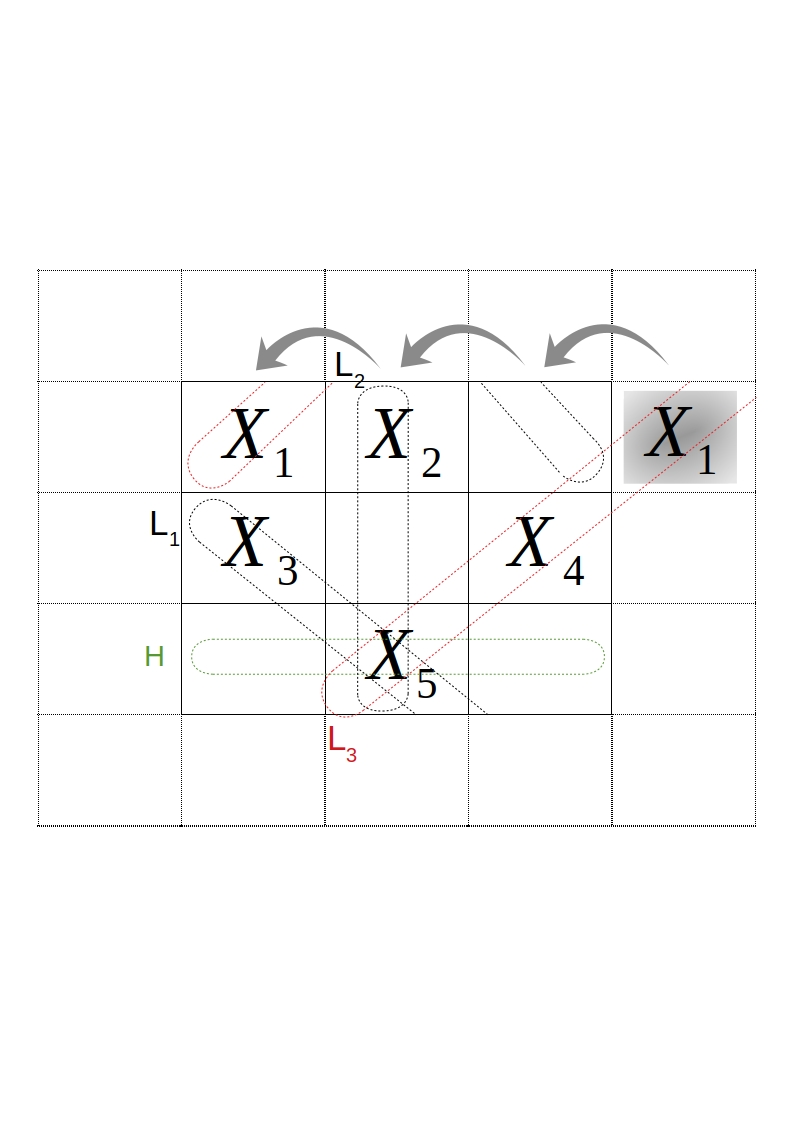
\includegraphics[width=0.5\textwidth]{Img/Fig2Prop1.jpg}
\caption{Les quatre lignes contenant le point $x_5$}
\end{figure}
    
Or la ligne $H$ ne contient aucun des points $x_1$ à $x_4$ donc selon le principe des tiroirs, il y a deux de ces points noté $x_r$ et $x_s$ qui se trouvent sur une ligne $L_i$ où $1\le i \le 3$.
Cela montre que la ligne $L_i$ contient les points $x_5, x_r, x_s$ formant donc un SET et cela contredit l'hypothèse de départ car un 2-cap est un sous espaces affine de $\mathbb{F}_3^2$ qui ne contient pas de points alignés (colinéaire).
%Lien vers le Wikipedia du principes des tiroirs :\\ \verb|https://fr.wikipedia.org/wiki/Principe_des_tiroirs|.   
\end{proof}

\subsubsection{Taille maximale d'un \emph{3-cap}}
\begin{prop} \label{prop:3cap}
La taille maximale d'un \emph{3-cap} est 9.
\end{prop}
\begin{proof}
Par l'absurde, supposons qu'il existe un 3-cap avec dix points. L'espace $\Ftrois{3}$ peut être décomposé comme l'union de trois plans parallèles.

Puisque l'intersection de n'importe quel plan avec le 3-cap est un 2-cap, la proposition \ref{prop:2cap} implique qu'aucun plan ne peut contenir plus de quatre points du cap. Cela signifie que le plan contenant le plus petit nombre de points doit contenir deux ou trois points, car s'il contenait quatre points, nous aurions besoin d'un total de douze points, et pour un point ou zéro cela signifierait au plus neuf points. Appelons  ce plan H, et notons qu’il y a au moins sept points du cap, $x_1,\dots ,x_7$, non contenu dans H.
    
Soient a et b deux points du cap sur le plan H. Il existe exactement quatre plans dans l'espace $\Ftrois{3}$ contenant à la fois a et b, que l'on désigne par $H, M_1, M_2, M_3$. Puisque H ne contient pas les points $x_1,\dots ,x_7$, selon le principe des tiroirs, l'un des plans $M_i$ doit contenir trois de ces points $x_r, x_s, x_t$. Cela montre que le plan $M_i$ contient un total de cinq points du cap, ce qui contredit la proposition \ref{prop:2cap}.
    
Malheureusement, cette méthode n'est pas assez puissante pour prouver que la taille maximale d'un \emph{4-cap} est 20.
\end{proof}

\subsubsection{Taille maximale d'un \emph{4-cap}}
Avant de commencer la démonstration, nous aurons besoin de la proposition suivante
\begin{prop} \label{prop:nbhyp}
Le nombre d'hyperplans contenant un sous-espace affine fixé de dimensions k dans $\Ftrois{d}$ est égal à :
\[
\frac{3^{d-k}-1}{2}
\]
\end{prop}
\begin{proof}
Soit S un sous-espace de $\Ftrois{d}$ de dimension k contenant l'origine. On peut dire que S est un sous-espace vectoriel de $\Ftrois{d}$ or $\Ftrois{d}$ est de dimension finie donc S admet un supplémentaire noté $G$ tel que $\Ftrois{d} = S \oplus G$.

L'application qui a chaque vecteur $y\in S$ associe sa classe d'équivalence $y + S$ est un isomorphisme entre $G$ et $\Ftrois{d}/S$. On en déduit qu'on a $\Ftrois{d}/S \simeq G \simeq \Ftrois{{d-k}}$.

Les hyperplans de $\Ftrois{{d-k}}$ contenant l'origine sont définis par un vecteur normal non nul au nombre de $3^{d-k}-1$. Comme il y a deux vecteurs normaux définissant un plan, il y a donc $\frac{3^{d-k}-1}{2}$ hyperplans contenant l'origine.
\begin{rmq}
Notons que si le sous espace fixé ne contient pas l'origine, il peut être translaté.
\end{rmq}
\end{proof}

\begin{prop}
La taille maximale d'un \emph{4-cap} est 20.
\end{prop}
\begin{proof}
Par l'absurde, supposons l'existence d'un \emph{4-cap} noté C contenant 21 points.
L'espace $\Ftrois{4}$ peut être décomposé de plusieurs façon comme l'union de trois hyperplans parallèles $H_1,H_2,H_3$.
On obtient alors un triplet 
\[ 
\{|C \cap H_1|,|C \cap H_2|,|C \cap H_3|\}
\]
où $|C \cap H_i|$ est la taille de $C \cap H_i$.

Soit $x_{ijk}$ le nombre de triplets d'hyperplans de C. D'après la proposition \ref{prop:3cap}, un \emph{3-cap} possède au maximum 9 points, il y a donc 7 triplets d'hyperplans possibles : 
\[
\{i,j,k\}=\{9,9,3\},\{9,8,4\},\{9,7,5\},\{9,6,6\},\{8,8,5\},\{8,7,6\},\{7,7,7\}
\]
De plus, pour une famille de trois hyperplans parallèles, il existe une unique droite passant par l'origine perpendiculaire à ces trois hyperplans. Le nombre de façon de décomposer $\Ftrois{4}$ comme l'union de trois hyperplans parallèles est alors égal à ce nombre de droites, c'est-à-dire égal à $\frac{3^{4}-1}{2}=40$, donc
\begin{equation} \label{eq:nbdecomp}
x_{993} + x_{984} + x_{975} + x_{966} + x_{885} + x_{876} + x_{777} = 40
\end{equation}
Pour obtenir une autre équation, nous allons compter le nombre de \emph{2-marked} hyperplans qui sont des paires de la forme $(H,\{x,y\} \subset H \cap C)$ où $H$ est un hyperplan. D'après la proposition \ref{prop:nbhyp}, le nombre d'hyperplans contenant une paire de points \textbf{fixé}, ou une ligne, est égal à $\frac{3^{4-1}-1}{2} = 13$. Il y a donc, $13 \binom{21}{2} = 2730$ \emph{2-marked} hyperplans. Par ailleurs, il y a 
\[
\left[\binom{9}{2}+\binom{9}{2}+\binom{3}{2}\right]x_{993} + \dots + \left[\binom{7}{2}+\binom{7}{2}+\binom{7}{2}\right]x_{777}
\]
\emph{2-marked} hyperplans. En calculant chacun des coefficients, on a
\begin{equation} \label{eq:nb2marked}
75x_{993} + 70x_{984} + 67x_{975} + 66x_{966} + 66x_{885} + 64x_{876} + 63x_{777} = 2730
\end{equation}

Pour obtenir encore une autre équation en $x_{ijk}$, nous allons compter le nombre de \emph{3-marked} hyperplans qui sont des paires de la forme $(H,\{x,y,z\} \subset H \cap C)$ où $H$ est un hyperplan. D'après la proposition \ref{prop:nbhyp}, le nombre d'hyperplans contenant trois points \textbf{fixé}, ou un plan, est égal à $\frac{3^{4-2}-1}{2} = 4$. Il y a donc, $4 \binom{21}{3} = 5320$ \emph{3-marked} hyperplans. Par ailleurs, il y a 
\[
\left[\binom{9}{3}+\binom{9}{3}+\binom{3}{3}\right]x_{993} + \dots + \left[\binom{7}{3}+\binom{7}{3}+\binom{7}{3}\right]x_{777}
\]
\emph{3-marked} hyperplans. En calculant chacun des coefficients, on a
\begin{equation} \label{eq:nb3marked}
169x_{993} + 144x_{984} + 129x_{975} + 124x_{966} + 122x_{885} + 111x_{876} + 105x_{777} = 5230
\end{equation}
Nous pouvons désormais résoudre les équations. Nous nous intéressons qu'aux solutions entières et positives. En ajoutant, 693 fois l'équation (\ref{eq:nbdecomp}) à 3 fois l'équation (\ref{eq:nb3marked}), et en soustrayant 6 fois l'équation (\ref{eq:nb2marked}), on a
\[
5x_{984} + 8x_{975} + 9x_{966} + 3x_{885} + 2x_{876} = 0
\]
Les uniques solution positives de cette équation sont $x_{984} = x_{975} = x_{966} = x_{885} = x_{876} = 0$. Mais l'équation (\ref{eq:nb2marked}) moins 63 fois l'équation (\ref{eq:nbdecomp}) donne
\[
12x_{993} + 7x_{984} + 4x_{975} + 3x_{966} + 3x_{885} + x_{876} = 210
\]
Finalement, on obtient $12x_{993} = 210$ qui contredit le fait que $x_{993}$ soit un entier.
\end{proof}

\section{Conclusion}
Nous avons vu que le jeu de SET pouvait se ramener à chercher trois points alignés dans $\Ftrois{4}$.
Parfois, il n'existe pas de set dans les cartes disposées devant soi, on se demandait alors combien de cartes faut il au minimum disposer devant soi pour être certain de trouver un set.
Pour répondre à cette question nous avons d'abord travaillé dans des sous-espaces vectoriels de $\Ftrois{4}$
et avons cherché les tailles maximales des \emph{d-cap}. Lors de nos recherches, nous avons trouvé ces résultats

\begin{center}
\begin{tabular}{ l | *{8}{c} }
d & 0 & 1 & 2 & 3 & 4 & 5 & 6 & 7\\
\hline
taille maximale & 1 & 2 & 4 & 9 & 20 & 45 & 112 & [236,291] \\
\end{tabular}
\end{center}

Il faut donc disposer au minimum 21 cartes pour être sûr de trouver un set.

\bibliographystyle{plain}
\bibliography{./Ref/davis2003.bib}

\end{document}